% Provenance (never printed): see sources/outline_sources.md (Year 3: rift
% models, normal-fault systems, metamorphic core complexes, strike-slip
% systems). Brief: sources/book5/BRIEFS.md, ch. 9. Curves from
% figdata/bachelor-3/domino_extension.py and rollover.py. Exercise and problem
% values in the Book 5 scratch calculator calc/ch09.py.
\chapter{Tectonique extensive et décrochante}\label{ch:b3:extension-strike-slip}

Entre la Sierra Nevada et le plateau du Colorado, des chaînons et des bassins
alternent comme les sillons d'un champ, chaque chaînon étant un bloc de croûte
basculé le long d'une faille normale. Dans les noyaux de certains de ces
chaînons, des roches enfouies entre \qty{23}{km} et \qty{30}{km} de profondeur,
entre \qty{500}{\celsius} et \qty{650}{\celsius}, affleurent aujourd'hui sous une
seule faille au pendage de quelques degrés seulement. Un continent peut être
étiré d'un facteur deux ou plus, et déchiré latéralement le long de failles qui
se coudent, se décalent et ouvrent des bassins profonds de \qty{10}{km}. Ce chapitre
construit la géométrie de l'extension et du décrochement, les quelques règles qui les gouvernent et les indices que laissent les systèmes réels.
% ledger: cooper10:snake-range, mcq05:basin-range, tb93:dead-sea-basin

\begin{recall}
Les failles normales, décrochantes et transformantes, le demi-graben et le rift
continental sont dans le volume de première année, dans ses chapitres sur les
rifts et sur les failles, plis et fabriques, avec la théorie d'Anderson~: avec $\sigma_1$ vertical, les failles normales
ont un pendage de $\ang{45} + \phi/2$, soit environ \ang{60}~; avec $\sigma_2$ vertical, les failles
décrochantes ont une direction faisant $\ang{45} - \phi/2$ avec $\sigma_1$. La loi de Byerlee sur le frottement des roches,
$\tau = 0.85\,\sigma_n$ en dessous de \qty{200}{MPa} et $\tau =
\qty{50}{MPa} + 0.6\,\sigma_n$ au-delà, figure dans son chapitre sur la contrainte, la déformation et la rhéologie. Le modèle
d'étirement, dans lequel la lithosphère est amincie uniformément d'un facteur $\beta$, et le bassin de rift sont dans le volume de deuxième année, dans son
chapitre consacré à la comparaison des bassins sédimentaires. Les \omterm{def:b3:deformation-mechanisms:shear-zone}{zones de
cisaillement} et les mylonites sont au
\cref{ch:b3:deformation-mechanisms}~; la profondeur du détachement à partir d'une aire en excès,
$A = Sh$, figure au \cref{ch:b3:structural-analysis}.
\end{recall}
% ledger: byerlee:1975

\section{Deux modèles de rift}\label{sec:b3:extension-strike-slip:models}

Le modèle d'étirement du volume de deuxième année amincit toute la lithosphère
du même facteur sous le même lieu~: croûte et manteau s'amincissent ensemble,
de façon symétrique, par cisaillement pur. Beaucoup de marges rifted ne sont
pas symétriques~: d'un côté s'étend une large région de blocs basculés, de l'autre une pente étroite et raide, et l'amincissement du manteau se situe
à côté, et non sous, celui de la croûte.

\begin{definition}[Modèle de rift en cisaillement simple]\label{def:b3:extension-strike-slip:rift-models}
Dans le \emph{modèle de rift en cisaillement simple}\index{modèle de rift en cisaillement simple}
la lithosphère est écartée le long d'une \omterm{def:b3:deformation-mechanisms:shear-zone}{zone de cisaillement} à faible pendage
qui la traverse depuis la surface jusqu'à sa base. La plaque située au-dessus
de la \omterm{def:b3:deformation-mechanisms:shear-zone}{zone de cisaillement}, la plaque supérieure, perd sa partie inférieure~;
la plaque située en dessous, la plaque inférieure, est retirée de sous elle.
L'amincissement de la croûte et celui du manteau sont décalés latéralement,
et les deux marges conjuguées qui se forment lorsque le continent se rompt sont asymétriques.
\end{definition}

Les rifts réels combinent les deux~: une fracturation fragile dans la croûte
supérieure, un amincissement ductile en dessous, et un manteau qui peut s'amincir
sur une région plus large ou plus étroite que la croûte (étirement dépendant
de la profondeur). Là où le manteau chaud remonte sous le rift, ou sous son flanc
dans le cas du cisaillement simple, la flottabilité soulève les épaules du rift, qui se dressent en montagnes au-dessus du fond du bassin.

\begin{omfigure}
\begin{tikzpicture}[scale=0.95, >=stealth]
% (a) pure shear
\begin{scope}
\fill[omLithBasalt!40] (0,-3.2) rectangle (6.6,-1.3);
\fill[omLithGranite!50] (0,0) -- (2.2,0) -- (2.5,-0.35) -- (4.1,-0.35) -- (4.4,0) -- (6.6,0) -- (6.6,-1.3)
  -- (4.4,-1.3) -- (3.3,-0.95) -- (2.2,-1.3) -- (0,-1.3) -- cycle;
\fill[omLithBasalt!40] (2.2,-1.3) -- (3.3,-0.95) -- (4.4,-1.3) -- cycle;
\fill[orange!25] (0,-3.2) -- (1.8,-3.2) -- (3.3,-2.1) -- (4.8,-3.2) -- (6.6,-3.2) -- (6.6,-3.7) -- (0,-3.7) -- cycle;
\draw (0,0) -- (2.2,0) -- (2.5,-0.35) -- (4.1,-0.35) -- (4.4,0) -- (6.6,0);
\draw (0,-1.3) -- (2.2,-1.3) -- (3.3,-0.95) -- (4.4,-1.3) -- (6.6,-1.3);
\draw (0,-3.2) -- (1.8,-3.2) -- (3.3,-2.1) -- (4.8,-3.2) -- (6.6,-3.2);
\draw[thick] (2.2,0) -- (2.75,-0.85); \draw[thick] (4.4,0) -- (3.85,-0.85);
\node[font=\scriptsize] at (0.7,-0.65) {croûte};
\node[font=\scriptsize, align=center] at (0.9,-2.25) {manteau\\ lithosphérique};
\node[font=\scriptsize] at (1.2,-3.48) {asthénosphère};
\draw[<-] (-0.1,0.25) -- (0.6,0.25); \draw[->] (6.0,0.25) -- (6.7,0.25);
\node[font=\small] at (3.3,-4.2) {(a) cisaillement pur};
\end{scope}
% (b) simple shear: crust thinned near the breakaway (left), mantle beneath the upper plate (right)
\begin{scope}[xshift=7.4cm]
\fill[omLithBasalt!40] (0,-3.2) rectangle (6.6,-1.3);
\fill[omLithGranite!50] (0,0) -- (0.9,0) -- (1.2,-0.3) -- (2.2,-0.3) -- (2.5,0) -- (4.0,0)
  .. controls (4.6,0.18) and (5.2,0.18) .. (5.8,0) -- (6.6,0) -- (6.6,-1.3)
  -- (2.9,-1.3) -- (2.0,-0.7) -- (1.2,-1.3) -- (0,-1.3) -- cycle;
\fill[omLithBasalt!40] (1.2,-1.3) -- (2.0,-0.7) -- (2.9,-1.3) -- cycle;
\fill[orange!25] (0,-3.2) -- (3.4,-3.2) -- (4.8,-2.1) -- (6.0,-3.2) -- (6.6,-3.2) -- (6.6,-3.7) -- (0,-3.7) -- cycle;
\draw (0,0) -- (0.9,0) -- (1.2,-0.3) -- (2.2,-0.3) -- (2.5,0) -- (4.0,0)
  .. controls (4.6,0.18) and (5.2,0.18) .. (5.8,0) -- (6.6,0);
\draw (0,-1.3) -- (1.2,-1.3) -- (2.0,-0.7) -- (2.9,-1.3) -- (6.6,-1.3);
\draw (0,-3.2) -- (3.4,-3.2) -- (4.8,-2.1) -- (6.0,-3.2) -- (6.6,-3.2);
\draw[omThm, very thick] (0.9,0) .. controls (2.4,-0.9) and (3.9,-1.8) .. (5.4,-3.2);
\node[font=\scriptsize, align=center] at (5.0,-0.6) {plaque supérieure};
\node[font=\scriptsize, align=center] at (1.3,-2.3) {plaque inférieure};
\node[omThm, font=\scriptsize, align=center] at (3.0,-2.15) {zone de\\ cisaillement};
\node[font=\scriptsize, align=center] at (4.9,0.42) {flanc soulevé};
\draw[<-] (-0.1,0.25) -- (0.6,0.25); \draw[->] (6.0,0.25) -- (6.7,0.25);
\node[font=\small] at (3.3,-4.2) {(b) cisaillement simple};
\end{scope}
\end{tikzpicture}

\par\smallskip{\small Deux modèles extrêmes de rift (non à l'échelle). (a) Cisaillement
pur~: croûte et manteau lithosphérique s'amincissent ensemble sous le rift, avec
des failles normales de part et d'autre. (b) Cisaillement simple~: une \omterm{def:b3:deformation-mechanisms:shear-zone}{zone de
cisaillement} à faible pendage traverse la lithosphère~; la croûte s'amincit près de
la trace de surface, le manteau du côté opposé, sous la plaque supérieure, de sorte que le rift est asymétrique et que son
flanc situé au-dessus du manteau aminci est soulevé.}\label{fig:b3:extension-strike-slip:models}
\end{omfigure}

\section{Systèmes de failles normales}\label{sec:b3:extension-strike-slip:faults}

\begin{definition}[Failles en dominos]\label{def:b3:extension-strike-slip:domino}
Dans les \emph{failles en dominos}\index{failles en dominos} un ensemble de failles normales planes
et parallèles découpe la croûte supérieure en blocs rigides qui, à mesure que la région
s'étire, basculent ensemble comme une rangée de livres qui tombent~: les failles
deviennent moins raides, et les couches, d'abord horizontales, basculent dans l'autre sens.
\end{definition}

\begin{theorem}[Extension en dominos]\label{thm:b3:extension-strike-slip:domino}
Soient des blocs rigides délimités par des failles planes et parallèles de pendage initial
$\theta_0$ qui tournent jusqu'à ce que les failles aient pour pendage $\theta$. Les couches ont alors un pendage de $\theta_0
- \theta$, en s'éloignant des failles, et la région a été étirée
d'un facteur
\[
  \beta = \frac{\sin\theta_0}{\sin\theta} .
\]
\end{theorem}

\begin{proof}
Les blocs étant rigides, la distance perpendiculaire $d$ entre deux
failles voisines ne change pas. Le long d'une horizontale, deux plans parallèles
de pendage $\theta$ et distants de $d$ découpent un segment de longueur $d/\sin
\theta$~; la largeur de la région varie comme la longueur de ce segment, de
$d/\sin\theta_0$ à $d/\sin\theta$. Les blocs tournent de l'angle dont
les failles se sont aplaties, $\theta_0 - \theta$, et les couches, horizontales
au départ, tournent avec elles.
\end{proof}

La rotation seule donne un étirement modeste~: des failles qui partent de \ang{60} et
s'aplatissent jusqu'à \ang{30} et étirent la région de $\beta = 1.73$. Elles ne peuvent
pas tourner indéfiniment~: une faille devient plus difficile à faire glisser à mesure qu'elle s'aplatit, car la
$\sigma_1$ verticale la comprime davantage et la cisaille moins.

\begin{proposition}[Verrouillage par frottement d'une faille normale]\label{prop:b3:extension-strike-slip:lockup}
Soit une faille sans cohésion, de coefficient de frottement $\mu$, qui fait un angle
$t$ avec $\sigma_1$, toutes les contraintes étant effectives. Elle glisse lorsque le \omterm{def:b3:structural-analysis:palaeostress}{rapport des
contraintes} principales atteint
\[
  \frac{\sigma_1}{\sigma_3} = \frac{1 + \mu\cot t}{1 - \mu\tan t} ,
\]
qui est minimal, $(\sqrt{1 + \mu^2} + \mu)^2$, pour $\tan2t = 1/\mu$, et
infini pour $\tan t = 1/\mu$. Avec $\sigma_1$ verticale, le pendage de la faille vaut
$\ang{90} - t$~: une faille normale de pendage inférieur à $\arctan\mu$ ne peut pas glisser
du tout.
\end{proposition}

\begin{proof}
Posons $m = (\sigma_1 + \sigma_3)/2$ et $s = (\sigma_1 - \sigma_3)/2$. Sur
le plan, $\sigma_n = \sigma_1\sin^2t + \sigma_3\cos^2t = m - s\cos2t$ et
$\tau = (\sigma_1 - \sigma_3)\sin t\cos t = s\sin2t$. Le glissement exige $\tau =
\mu\sigma_n$~; en divisant par $\sigma_3\sin t\cos t$ et en regroupant $\sigma_1$
donne le rapport, dont le dénominateur s'annule pour $\tan t = 1/\mu$. Sous l'autre
forme, la condition s'écrit $s(\sin2t + \mu\cos2t) = \mu m$. Le crochet vaut au
plus $\sqrt{1 + \mu^2}$, atteint pour $\tan2t = 1/\mu$, où le glissement exige le
plus petit $s/m = \mu/\sqrt{1 + \mu^2}$~; alors $\sigma_1/\sigma_3 = (m + s)/(m - s) =
(\sqrt{1 + \mu^2} + \mu)/(\sqrt{1 + \mu^2} - \mu) = (\sqrt{1 + \mu^2} +
\mu)^2$, car le produit des deux derniers facteurs vaut 1.
\end{proof}

Avec $\mu = 0.6$ de Byerlee, la faille normale la mieux orientée a un pendage de \ang{60.5} et
glisse lorsque $\sigma_1 = 3.12\,\sigma_3$~; une faille à \ang{45} exige $4.0$, et
aucune faille de pendage inférieur à \ang{31} ne glisse~; avec $\mu = 0.85$, le pendage de verrouillage est
\ang{40}. La figure ci-dessous montre les deux résultats. Lorsqu'un ensemble de \omterm{def:b3:extension-strike-slip:domino}{failles en dominos} approche
du verrouillage, un nouvel ensemble de failles raides recoupe l'ancien~: les régions fortement étirées
montrent plusieurs générations de failles.

\begin{omfigure}
\begin{tikzpicture}
\begin{groupplot}[group style={group size=2 by 1, horizontal sep=1.6cm},
  omrecord, width=0.47\linewidth, height=0.42\linewidth, title style={font=\small},
  legend style={font=\scriptsize, legend cell align=left}]
\nextgroupplot[title={(a) extension par dominos rigides}, xlabel={pendage actuel des failles $\theta$ (\unit{\degree})},
  ylabel={facteur d'étirement $\beta$}, xmin=10, xmax=70, ymin=1, ymax=4,
  legend style={at={(0.97,0.97)}, anchor=north east}]
% computed in figdata/bachelor-3/domino_extension.py
\addplot[omDef, thick] table[x=dip, y=b70] {figdata/out/bachelor-3-domino_extension-beta.dat};
\addlegendentry{$\theta_0 = \ang{70}$}
\addplot[red!70!black, thick, densely dashed] table[x=dip, y=b60] {figdata/out/bachelor-3-domino_extension-beta.dat};
\addlegendentry{$\theta_0 = \ang{60}$}
\addplot[black, thick, densely dotted] table[x=dip, y=b45] {figdata/out/bachelor-3-domino_extension-beta.dat};
\addlegendentry{$\theta_0 = \ang{45}$}
\nextgroupplot[title={(b) rapport de contraintes nécessaire au glissement}, xlabel={pendage de la faille (\unit{\degree})},
  ylabel={$\sigma_1/\sigma_3$}, xmin=20, xmax=90, ymode=log, ymin=1, ymax=40,
  log ticks with fixed point, ytick={1,2,5,10,20,40},
  legend style={at={(0.97,0.97)}, anchor=north east}]
\addplot[omDef, thick] table[x=dip, y=r060] {figdata/out/bachelor-3-domino_extension-lockup.dat};
\addlegendentry{$\mu = 0.6$}
\addplot[red!70!black, thick, densely dashed] table[x=dip, y=r085] {figdata/out/bachelor-3-domino_extension-lockup.dat};
\addlegendentry{$\mu = 0.85$}
\end{groupplot}
\end{tikzpicture}

\par\smallskip{\small (a) Facteur d'étirement d'un domaine de dominos rigides lorsque
ses failles tournent depuis le pendage initial $\theta_0$ jusqu'à $\theta$. (b) \omterm{def:b3:structural-analysis:palaeostress}{Rapport des
contraintes} principales effectives nécessaires pour faire glisser une faille normale d'un pendage donné
sous une contrainte $\sigma_1$ verticale, pour les deux coefficients de frottement de Byerlee~: minimal
vers \ang{60} et \ang{65}, infini aux pendages de verrouillage \ang{31} et
\ang{40}.}\label{fig:b3:extension-strike-slip:domino}
\end{omfigure}

De nombreuses grandes failles normales sont courbes, raides en surface et s'aplatissant en
profondeur pour devenir une faille ou une \omterm{def:b3:deformation-mechanisms:shear-zone}{zone de cisaillement} presque horizontale.

\begin{definition}[Faille de détachement, faille listrique, anticlinal de roll-over]\label{def:b3:extension-strike-slip:detachment}
Une \emph{faille de détachement}\index{faille de détachement} est une faille normale à faible
pendage ou \omterm{def:b3:deformation-mechanisms:shear-zone}{zone de cisaillement} à grand déplacement, de quelques kilomètres à quelques dizaines de kilomètres, qui
sépare un compartiment supérieur étiré d'un compartiment inférieur déformé différemment. Une
\emph{faille listrique}\index{faille listrique} est une faille normale dont le pendage
diminue avec la profondeur, son profil étant concave vers le haut. Lorsque le toit d'une
faille listrique s'abaisse et s'éloigne, il se courbe pour rester en contact avec la
faille~: ses couches basculent vers la faille dans un large pli, le \emph{anticlinal de
roll-over}\index{anticlinal de roll-over}.
\end{definition}

\begin{method}[Construction à rejet horizontal constant]\label{met:b3:extension-strike-slip:heave}
Pour tracer le toit d'une \omterm{def:b3:extension-strike-slip:detachment}{faille listrique} après un déplacement horizontal
$H$, soit le rejet horizontal, sur une coupe parallèle au glissement~:
\begin{enumerate}
  \item Diviser le toit en colonnes verticales. Déplacer chaque colonne
        latéralement de $H$, en s'éloignant du mur.
  \item Abaisser chaque colonne du dénivelé de la faille située sous elle~: une colonne qui
        part d'un point où la faille se trouve à la profondeur $f(x)$ et finit là où elle
        se trouve à $f(x + H)$ descend de $f(x + H) - f(x)$, ce qui ramène sa base
        sur la faille.
  \item L'espace laissé entre le mur et le toit déplacé est le
        demi-graben, comblé au fur et à mesure de son ouverture par des sédiments qui s'épaississent vers la
        faille.
\end{enumerate}
Lu à rebours, la construction restaure la coupe et prédit la forme
de la faille à partir de la forme du roll-over.
\end{method}

L'aire située sous le niveau d'origine d'un banc, comptée à partir de la faille, est
l'aire du \cref{ch:b3:structural-analysis} au signe près~: $A =
H(D - z_0)$ pour un banc situé d'abord à la profondeur $z_0$ au-dessus d'un décollement à la
profondeur $D$, puisque la roche sous le banc conserve son aire tandis que sa longueur croît de
$H$. Mesurer $A$ et $H$ sur une coupe sismique donne la profondeur du
décollement. La figure ci-dessous illustre la construction.

\begin{omfigure}
\begin{tikzpicture}
\begin{axis}[width=0.9\linewidth, height=0.36\linewidth, omsection,
  xmin=-2, xmax=24, ymin=0, ymax=6, y dir=reverse,
  xlabel={distance (\unit{km})}, ylabel={profondeur (\unit{km})},
  legend style={font=\scriptsize, legend cell align=left, at={(0.98,0.27)}, anchor=south east}]
% computed in figdata/bachelor-3/rollover.py (heave 2 km, detachment at 5 km)
\addplot[name path=fault, black, very thick] table[x=x, y=z] {figdata/out/bachelor-3-rollover-fault.dat};
\addlegendentry{faille listrique}
\addplot[name path=top, omDef, thick] table[x=x, y=z] {figdata/out/bachelor-3-rollover-top.dat};
\addlegendentry{sommet du toit}
\addplot[omDef, thick, densely dashed] table[x=x, y=z] {figdata/out/bachelor-3-rollover-bed.dat};
\addlegendentry{un banc situé d'abord à \qty{2}{km}}
\addplot[gray, dashed, forget plot] coordinates {(-2,0) (24,0)};
\addplot[gray, dashed, forget plot] coordinates {(-2,5) (24,5)};
\node[font=\scriptsize, anchor=west] at (axis cs:15,5.35) {décollement};
\node[font=\scriptsize] at (axis cs:3.9,0.45) {demi-graben};
\node[font=\scriptsize] at (axis cs:-1,1.5) {mur};
\node[font=\scriptsize] at (axis cs:9.5,1.15) {roll-over};
\end{axis}
\end{tikzpicture}

\par\smallskip{\small \omterm{def:b3:extension-strike-slip:detachment}{Faille listrique} au pendage de \ang{60} en surface et
s'aplatissant en un décollement à \qty{5}{km}, après un rejet horizontal de \qty{2}{km}
tracé par la construction à rejet constant. Le sommet du toit et un
banc plus profond s'incurvent vers la faille en un roll-over~; l'aire située sous le
toit d'origine, \qty{10}{km^2}, est le rejet multiplié par la profondeur du décollement, et sous
le banc profond \qty{6}{km^2}, le rejet multiplié par sa hauteur au-dessus de celui-ci.}\label{fig:b3:extension-strike-slip:rollover}
\end{omfigure}

Les failles normales ne sont pas infinies. Là où une faille s'éteint le long de la direction, son
déplacement passe à une autre, souvent de pendage opposé, et les demi-grabens d'un rift
alternent de polarité sur toute sa longueur.

\begin{definition}[Zone de transfert]\label{def:b3:extension-strike-slip:transfer}
Une \emph{zone de transfert}\index{zone de transfert} est la région comprise entre deux
segments de faille normale, ou deux segments de rift, qui se chevauchent ou sont décalés, et
à travers laquelle l'extension passe de l'un à l'autre~: une rampe relais entre deux failles
de même polarité, un haut entre deux demi-grabens de polarité opposée, ou une faille
décrochante, la faille de transfert, parallèle à l'extension.
\end{definition}

\section{Core complexes métamorphiques}\label{sec:b3:extension-strike-slip:core}

\begin{definition}[Core complex métamorphique, charnière roulante]\label{def:b3:extension-strike-slip:core-complex}
Un \emph{core complex métamorphique}\index{core complex métamorphique} est un dôme de
roches métamorphiques et de mylonites, remonté depuis la croûte moyenne ou inférieure,
sous une \omterm{def:b3:extension-strike-slip:detachment}{faille de détachement} dont le compartiment supérieur est une mosaïque de blocs
basculés de roches de croûte supérieure. Dans le modèle de \emph{charnière roulante}\index{charnière roulante},
le détachement glisse selon un pendage modéré en profondeur~; à mesure que le compartiment
supérieur s'éloigne, le mur déchargé remonte par isostasie et se courbe, de sorte que chaque
partie de la faille tourne vers un faible pendage, et cesse de glisser, une fois passée par
une charnière qui migre avec l'extension.
\end{definition}

Les mylonites du mur enregistrent la partie profonde de l'histoire~: elles constituent la \omterm{def:b3:deformation-mechanisms:shear-zone}{zone de
cisaillement} du \cref{ch:b3:deformation-mechanisms}, et leurs \omterm{def:b3:deformation-mechanisms:kinematic}{indicateurs cinématiques} donnent le
sens de transport du compartiment supérieur. Plus haut, les mêmes roches traversent la
transition cassant--ductile et sont surimprimées par des
cataclasites et des brèches juste sous la faille. Dans le nord de la chaîne Snake
au Nevada, des schistes à grenat du mur ont atteint 6 à \qty{8}{kbar}
et 500 à \qty{650}{\celsius}, soit des profondeurs d'enfouissement de 23 à \qty{30}{km}~; le
détachement qui les a remontés est interprété comme une \omterm{def:b3:extension-strike-slip:core-complex}{charnière roulante}.
% ledger: cooper10:snake-range

\begin{omfigure}
\begin{tikzpicture}[scale=1.0, >=stealth]
% upper plate dominoes on the left
\foreach \x in {0.0,0.9,1.8} {
  \fill[omLithSand] (\x,0) -- (\x+0.8,0) -- (\x+1.3,-0.9+0.25*\x) -- (\x+0.4,-1.5+0.2*\x) -- cycle;
  \draw (\x,0) -- (\x+0.8,0) -- (\x+1.3,-0.9+0.25*\x) -- (\x+0.4,-1.5+0.2*\x) -- cycle;
}
\fill[omLithGranite!45] (0,-2.6) -- (0,-1.6) .. controls (2.5,-1.2) and (4.0,-0.15) .. (6.0,-0.1)
  .. controls (8.0,-0.15) and (9.5,-0.9) .. (11.2,-1.0) -- (11.2,-2.6) -- cycle;
\fill[pattern=horizontal lines, pattern color=gray] (0,-1.6) .. controls (2.5,-1.2) and (4.0,-0.15) .. (6.0,-0.1)
  .. controls (8.0,-0.15) and (9.5,-0.9) .. (11.2,-1.0) -- (11.2,-1.35)
  .. controls (9.5,-1.25) and (8.0,-0.5) .. (6.0,-0.45) .. controls (4.0,-0.5) and (2.5,-1.55) .. (0,-1.95) -- cycle;
\draw[omThm, very thick] (0,-1.6) .. controls (2.5,-1.2) and (4.0,-0.15) .. (6.0,-0.1)
  .. controls (8.0,-0.15) and (9.5,-0.9) .. (11.2,-1.0);
% upper plate to the right, still in place
\fill[omLithSand] (8.4,0) -- (11.2,0) -- (11.2,-1.0) .. controls (10.2,-0.95) and (9.3,-0.75) .. (8.4,-0.35) -- cycle;
\draw (8.4,0) -- (11.2,0); \draw (8.4,0) -- (8.4,-0.35);
\node[font=\scriptsize] at (9.9,-0.45) {plaque supérieure};
\node[font=\scriptsize] at (1.5,0.3) {blocs basculés};
\node[omThm, font=\scriptsize] at (6.0,0.15) {détachement};
\node[font=\scriptsize] at (6.0,-0.75) {mylonites};
\node[font=\scriptsize, align=center] at (6.0,-1.8) {mur de croûte\\ moyenne};
\draw[->, thick] (6.0,-2.9) -- (6.0,-2.2) node[pos=0, below, font=\scriptsize] {remontée isostatique};
\draw[->, omThm] (10.4,0.3) -- (11.1,0.3);
\draw[->, omThm] (1.0,0.55) -- (0.3,0.55);
\draw[dashed] (7.6,-0.3) -- (8.6,-1.5) node[below, font=\scriptsize] {charnière roulante};
\end{tikzpicture}

\par\smallskip{\small Anatomie d'un \omterm{def:b3:extension-strike-slip:core-complex}{core complex métamorphique} (non à l'échelle).
Le mur du détachement, un dôme de roches de croûte moyenne surmonté d'une carapace de
mylonites, remonte sous la plaque supérieure à mesure qu'elle est écartée des deux côtés~;
la partie du détachement qui a dépassé la \omterm{def:b3:extension-strike-slip:core-complex}{charnière roulante} a été courbée vers un faible
pendage et ne glisse plus. Des blocs basculés de la plaque supérieure reposent sur le
détachement.}\label{fig:b3:extension-strike-slip:core}
\end{omfigure}

Les faibles pendages constituent un paradoxe~: d'après la proposition de blocage, aucune faille
normale de pendage inférieur à environ \ang{31} ne devrait glisser sous un $\sigma_1$ vertical
avec le frottement de Byerlee. La \omterm{def:b3:extension-strike-slip:core-complex}{charnière roulante} est une issue possible~: la partie active de la
faille est plus raide que ce qu'on observe. Les autres sont une faille affaiblie par des argiles
ou par des fluides à haute pression, ce qui abaisse le $\mu$ effectif, ou un champ de contraintes
tourné près d'une \omterm{def:b3:deformation-mechanisms:shear-zone}{zone de cisaillement} en profondeur~; les séismes sur les failles normales à faible
angle sont rares, ce qui favorise un glissement en pente forte ou un glissement sans séisme.

\section{Systèmes décrochants}\label{sec:b3:extension-strike-slip:strike-slip}

Dans les expériences sur gâteau d'argile comme dans la nature, une faille décrochante ne découpe pas
un plan net à travers une couverture sédimentaire~: elle croît en une bande de courtes
fractures en échelon aux angles constants.

\begin{definition}[Cisaillement de Riedel]\label{def:b3:extension-strike-slip:riedel}
Dans une \omterm{def:b3:deformation-mechanisms:shear-zone}{zone de cisaillement} simple décrochant, \emph{fractures de Riedel}\index{fractures de Riedel}
sont les courtes fractures de cisaillement qui se forment en premier, en deux familles~: les fractures R,
à faible angle par rapport à la zone et de même sens de glissement, et les fractures R$'$,
à grand angle et de sens opposé. Plus tard, les fractures P, symétriques
des fractures R par rapport à la zone, et les fractures de tension T complètent la figure.
\end{definition}

\begin{proposition}[Angles de Riedel]\label{prop:b3:extension-strike-slip:riedel}
Dans une \omterm{def:b3:deformation-mechanisms:shear-zone}{zone de cisaillement} simple, $\sigma_1$ est situé dans le plan horizontal à
\ang{45} de la zone. Pour une roche qui se rompt selon le critère de Coulomb, avec l'angle
de frottement interne $\phi$, les fractures R forment avec la zone un angle $\phi/2$, les
fractures R$'$ un angle $\ang{90} - \phi/2$, tous deux mesurés depuis la zone
du côté de $\sigma_1$, et les fractures de tension se forment parallèlement à $\sigma_1$,
à \ang{45}.
\end{proposition}

\begin{proof}
En cisaillement simple, les directions principales de la déformation infinitésimale sont à
\ang{45} du plan de cisaillement, et un matériau isotrope est soumis à
$\sigma_1$ selon la direction de raccourcissement. D'après le théorème d'Anderson, les deux plans de Coulomb
contiennent $\sigma_2$, vertical ici, et font $\ang{45} - \phi/2$ avec
$\sigma_1$ de part et d'autre~: celui le plus proche de la zone à $\ang{45} -
(\ang{45} - \phi/2) = \phi/2$ de celle-ci, l'autre à $\ang{45} + \ang{45} -
\phi/2$. Chacun glisse de façon à raccourcir selon $\sigma_1$~: la fracture R avec la
zone, la fracture R$'$ en sens inverse. Les fractures de tension s'ouvrent contre $\sigma_3$ et
se placent perpendiculairement à celui-ci.
\end{proof}

Pour $\phi = \ang{30}$, les fractures R sont à \ang{15} et les fractures R$'$ à
\ang{75}. Lorsque la faille principale n'est pas rectiligne, les blocs de part et d'autre
convergent ou divergent en la traversant.

\begin{definition}[Coude compressif, coude extensif]\label{def:b3:extension-strike-slip:bends}
Un coude ou un décrochement d'une faille décrochante est un \emph{coude
compressif}\index{coude compressif} lorsque le mouvement des blocs les rapproche
en la traversant, et un \emph{coude extensif}\index{coude extensif} lorsqu'il
les écarte. Pour une faille dextre, un décrochement vers la droite est extensif et un
décrochement vers la gauche compressif~; pour une faille senestre, c'est l'inverse.
\end{definition}

\begin{definition}[Bassin en pull-apart]\label{def:b3:extension-strike-slip:pull-apart}
Un \emph{bassin en pull-apart}\index{bassin en pull-apart} est un bassin qui s'ouvre à un
décrochement extensif entre deux segments de faille décrochante qui se recouvrent, bordé par
ces segments le long de ses grands côtés et par des failles normales obliques à ses extrémités.
Sa surface croît comme la largeur du décrochement multipliée par le rejet de la faille.
\end{definition}

\begin{definition}[Structure en fleur]\label{def:b3:extension-strike-slip:flower}
Une \emph{structure en fleur}\index{structure en fleur} est l'éventail de branches de faille,
vu sur une coupe, dans lequel une faille décrochante verticale se divise en approchant
de la surface~: une structure en fleur positive, dont les branches ont une composante inverse
et soulèvent une crête, au niveau d'un \omterm{def:b3:extension-strike-slip:bends}{coude compressif}~; une structure en fleur négative, dont les branches ont
une composante normale et encadrent une dépression, au niveau d'un \omterm{def:b3:extension-strike-slip:bends}{coude extensif}.
\end{definition}

\begin{definition}[Transpression et transtension]\label{def:b3:extension-strike-slip:transpression}
La \emph{transpression}\index{transpression} est une déformation décrochante combinée
à un raccourcissement perpendiculaire à la zone~; la \emph{transtension}\index{transtension},
une déformation décrochante combinée à une extension perpendiculaire à celle-ci. Les deux apparaissent lorsque
le mouvement entre deux blocs est oblique à la limite qui les sépare.
\end{definition}

Le mouvement oblique est souvent partitionné~: une faille décrochante reprend le mouvement
parallèle à la limite, tandis que des chevauchements ou des plis situés à côté, ou des failles normales,
reprennent le mouvement qui la traverse.

\begin{omfigure}
\begin{tikzpicture}[scale=1.0, >=stealth]
% (a) Riedel geometry, dextral E-W zone
\begin{scope}
\draw[thick] (0,0.9) -- (5,0.9); \draw[thick] (0,-0.9) -- (5,-0.9);
\draw[->] (1.0,1.15) -- (2.0,1.15); \draw[->] (4.0,-1.15) -- (3.0,-1.15);
\foreach \x in {0.6,1.6,2.6,3.6} \draw[omDef, thick] (\x,0.2) -- ++(-15:0.9);
\node[omDef, font=\scriptsize] at (4.6,0.05) {R};
\foreach \x in {1.0,2.4} \draw[red!70!black, thick] (\x,-0.6) -- ++(105:0.75);
\node[red!70!black, font=\scriptsize] at (1.0,-0.75) {R$'$};
\foreach \x in {3.3,3.7,4.1} \draw[black, thick] (\x,-0.25) -- ++(15:0.45);
\node[font=\scriptsize] at (4.6,-0.35) {P};
\foreach \x in {0.5,0.9} \draw[omMeth, line width=1.4pt] (\x,0.45) -- ++(135:0.35);
\node[omMeth, font=\scriptsize] at (0.25,0.25) {T};
\draw[<->, omThm] ($(2.6,0)+(135:0.55)$) -- ($(2.6,0)+(-45:0.55)$);
\node[omThm, font=\scriptsize] at (2.05,0.62) {$\sigma_1$};
\node[font=\small] at (2.5,-1.6) {(a) fractures de Riedel, dextre};
\end{scope}
% (b) releasing and restraining steps on a dextral fault
\begin{scope}[xshift=6.0cm]
\fill[omLithSand!70] (1.6,0.75) -- (2.6,0.75) -- (2.6,0.25) -- (1.6,0.25) -- cycle;
\draw[thick] (0,0.75) -- (2.6,0.75); \draw[thick] (1.6,0.25) -- (4.2,0.25);
\draw[->] (0.3,1.0) -- (1.0,1.0); \draw[->] (3.9,0.0) -- (3.2,0.0);
\node[font=\scriptsize] at (2.1,0.5) {bassin};
\node[font=\scriptsize, anchor=west] at (2.75,0.95) {extensif};
\fill[omLithGranite!60] (1.6,-0.65) -- (2.6,-0.65) -- (2.6,-1.15) -- (1.6,-1.15) -- cycle;
\draw[thick] (0,-1.15) -- (2.6,-1.15); \draw[thick] (1.6,-0.65) -- (4.2,-0.65);
\draw[->] (0.3,-0.9) -- (1.0,-0.9); \draw[->] (3.9,-0.9) -- (3.2,-0.9);
\node[font=\scriptsize] at (2.1,-0.9) {crête};
\node[font=\scriptsize, anchor=west] at (2.75,-0.45) {compressif};
\node[font=\small] at (2.1,-1.6) {(b) décrochements, dextre, carte};
\end{scope}
% (c) flower structures in section
\begin{scope}[xshift=11.0cm]
\draw[thick] (1.0,-1.3) -- (1.0,-0.4);
\draw[thick] (1.0,-0.4) .. controls (0.9,0.1) .. (0.45,0.8);
\draw[thick] (1.0,-0.4) -- (1.0,0.8);
\draw[thick] (1.0,-0.4) .. controls (1.1,0.1) .. (1.55,0.8);
\draw (0.0,0.8) -- (0.45,0.8) .. controls (0.8,1.1) and (1.2,1.1) .. (1.55,0.8) -- (2.0,0.8);
\node[font=\scriptsize, align=center] at (1.0,-1.6) {positive};
\draw[thick] (3.2,-1.3) -- (3.2,-0.4);
\draw[thick] (3.2,-0.4) .. controls (3.1,0.1) .. (2.65,0.8);
\draw[thick] (3.2,-0.4) -- (3.2,0.8);
\draw[thick] (3.2,-0.4) .. controls (3.3,0.1) .. (3.75,0.8);
\draw (2.2,0.8) -- (2.65,0.8) .. controls (3.0,0.5) and (3.4,0.5) .. (3.75,0.8) -- (4.2,0.8);
\node[font=\scriptsize, align=center] at (3.2,-1.6) {négative};
\node[font=\small] at (2.1,-1.95) {(c) fleurs, coupe};
\end{scope}
\end{tikzpicture}

\par\smallskip{\small Structures de décrochement (non à l'échelle). (a) Dans une
zone dextre, $\sigma_1$ à \ang{45}~: cisaillements R à \ang{15} et P à
\ang{-15} de même sens que la zone, cisaillements R$'$ à \ang{75} de sens
opposé, fractures de tension T parallèles à $\sigma_1$. (b) Un relais à droite sur une
faille dextre ouvre un \omterm{def:b3:extension-strike-slip:pull-apart}{bassin en pull-apart}~; un relais à gauche soulève une crête. (c) La
faille se divise vers le haut en une \omterm{def:b3:extension-strike-slip:flower}{structure en fleur} positive sous une crête et une
\omterm{def:b3:extension-strike-slip:flower}{structure en fleur} négative sous une dépression.}\label{fig:b3:extension-strike-slip:strike-slip}
\end{omfigure}

\section{Trois systèmes}\label{sec:b3:extension-strike-slip:systems}

\paragraph{Le Basin and Range.} Une reconstruction de la région depuis
\qty{36}{Ma} donne environ \qty{235}{km} d'extension, orientée vers
N\ang{78}O, aussi bien au nord, où elle atteint \qty{50}{\percent}, qu'au
centre, où elle atteint \qty{200}{\percent}~: la partie centrale est trois
fois plus large qu'auparavant. Depuis 10 à \qty{12}{Ma}, une partie du
mouvement décrochant dextre de la limite Pacifique--Amérique du Nord s'est
transférée dans le continent, sur environ \qty{100}{km} orientés N\ang{25}O, à environ \qty{1}{cm/an}~: la région est
désormais en \omterm{def:b3:extension-strike-slip:transpression}{transtension}. Ses core complexes se situent là où l'extension a été la plus forte.
% ledger: mcq05:basin-range

\paragraph{La mer Morte.} La faille transformante de la mer Morte a accumulé
environ \qty{105}{km} de mouvement senestre entre l'Afrique et l'Arabie depuis
environ \qty{20}{Ma}. Le long de celle-ci, le bassin de la mer Morte est un pull-apart \qty{132}{km}
de long, large de 7 à \qty{10}{km} et profond jusqu'à \qty{10}{km}, bordé sur
ses flancs par des failles subverticales~; les modèles gravimétriques donnent \qty{21}{km} d'étirement
selon son axe, soit un facteur de 1.19, ce qui, au rythme de la plaque de
\qty{6}{mm/an}, demande environ \qty{3.5}{Ma}. Ailleurs sur la transformante, un
segment présente une \omterm{def:b3:extension-strike-slip:flower}{structure en fleur} positive large de 100 à \qty{300}{m} dans la
partie supérieure, sur quelques centaines de mètres, et d'autres petits pull-aparts.
% ledger: weber09:dst, tb93:dead-sea-basin

\paragraph{La faille de San Andreas.} Le système de failles mesure plus de \qty{1290}{km}
(800 miles) de long~; il a parcouru au moins \qty{560}{km} (350 miles) depuis
sa formation, il y a 15 à \qty{20}{Ma}, et les mesures indiquent une dérive pouvant atteindre environ
\qty{5}{cm/an} (2 pouces par an). Là où elle s'infléchit au nord de Los Angeles, le
mouvement est oblique à la faille~: les blocs situés dans et à proximité de la zone de faille, dans
les monts San Bernardino se sont soulevés de 3 à \qty{4}{km} ou davantage, à
\qty{1.5}{mm/an} ou plus, par convergence et partition du glissement de
la \omterm{def:b3:extension-strike-slip:transpression}{transpression}.
% ledger: usgs:saf, sp98:san-bernardino

\begin{inthefield}[Cartographier une faille de détachement]
\begin{minipage}[t]{0.55\linewidth}\vspace{0pt}
Sur un core complex, le détachement forme souvent la surface lisse et
faiblement inclinée du relief lui-même, là où l'érosion a décapé le compartiment supérieur. Les
géologues qui le cartographient suivent le contact entre les roches fragiles du
compartiment supérieur et les mylonites sous-jacentes, relèvent son attitude tous les quelques centaines de
mètres au stéréonet, et mesurent les linéations sur la surface de faille et dans
les mylonites~: leur azimut donne la direction du transport, leurs \omterm{def:b3:deformation-mechanisms:kinematic}{indicateurs
cinématiques} le sens. Des échantillons du mur sont envoyés au laboratoire pour
la géobarométrie et pour des âges sur minéraux qui datent son refroidissement~; les
blocs du compartiment supérieur sont cartographiés pour l'inclinaison de leurs couches, qui
enregistre de combien leurs failles ont basculé.
\end{minipage}\hfill
\begin{minipage}[t]{0.42\linewidth}\vspace{0pt}
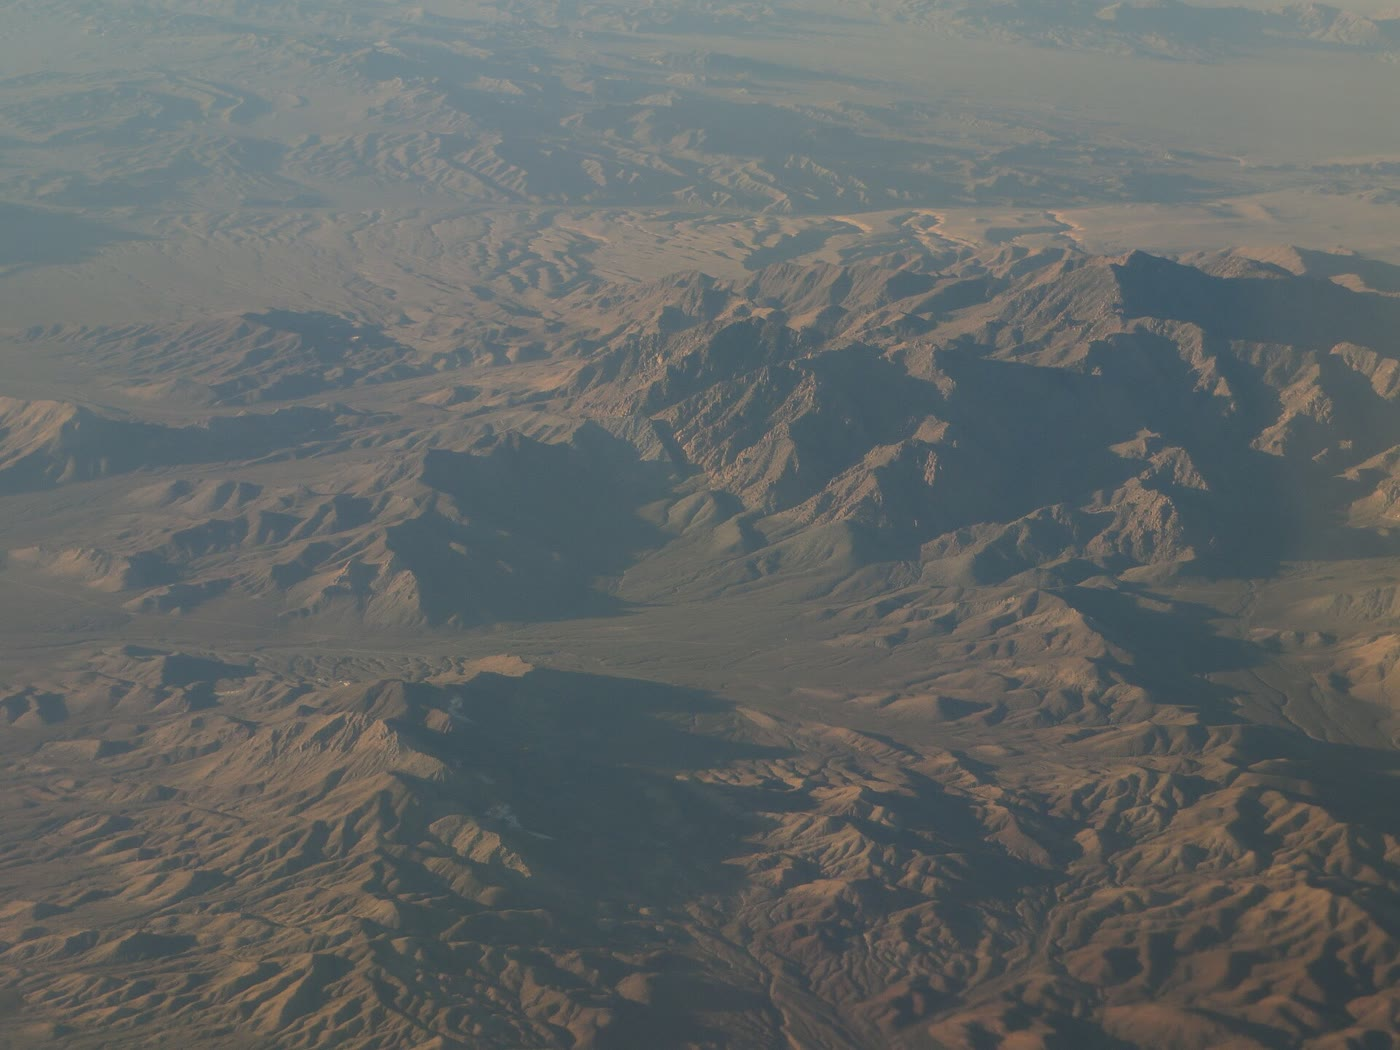
\includegraphics[width=\linewidth]{images/book5/b3-basin-and-range.jpg}

{\scriptsize Topographie de type Basin and Range au sud de Death Valley, Californie,
vue aérienne~: chaînons parallèles de blocs basculés séparés par des
bassins remplis de sédiments. Photo Ken Lund, CC BY-SA 2.0.}
\end{minipage}
\end{inthefield}
% ledger: photo:b3-basin-and-range

\section{Exercices}

\begin{exercise}[$\star$]\label{exo:b3:extension-strike-slip:1}
Pour un domaine de dominos rigides dont les failles plongent à \ang{35}~; elles se sont formées à
\ang{50}, calculer le pendage des couches et le facteur d'extension.
\end{exercise}

\begin{exercise}[$\star$]\label{exo:b3:extension-strike-slip:2}
Dire si chaque relais ouvre un bassin ou soulève une crête~: une faille dextre
qui fait un relais à droite~; une faille dextre qui fait un relais à gauche~; une faille senestre qui fait
un relais à gauche~; une faille senestre qui fait un relais à droite.
\end{exercise}

\begin{exercise}[$\star$]\label{exo:b3:extension-strike-slip:3}
La faille transformante de la mer Morte a parcouru \qty{105}{km} en environ \qty{20}{Ma}.
Calculer la vitesse moyenne en \unit{mm/an} et la comparer aux \qty{6}{mm/an}
utilisés pour le bassin de la mer Morte.
\end{exercise}

\begin{exercise}[$\star$]\label{exo:b3:extension-strike-slip:4}
Dans le centre du Basin and Range, \qty{235}{km} d'extension correspondent à
\qty{200}{\percent}. Calculer la largeur de la région avant et après. Faire
de même pour la partie nord, à \qty{50}{\percent}.
\end{exercise}

\begin{exercise}[$\star\star$]\label{exo:b3:extension-strike-slip:5}
La faille de San Andreas a parcouru au moins \qty{563}{km} en 15 à
\qty{20}{Ma}. Calculer l'intervalle des vitesses moyennes et les comparer à une
dérive actuelle d'environ \qty{51}{mm/an}. Qu'est-ce qui pourrait expliquer la différence~?
\end{exercise}

\begin{exercise}[$\star\star$]\label{exo:b3:extension-strike-slip:6}
Avec $\mu = 0.6$, calculer le rapport $\sigma_1/\sigma_3$ nécessaire pour faire glisser des failles normales
plongeant à \ang{60}, \ang{50} et \ang{40}, ainsi que le pendage de blocage.
\end{exercise}

\begin{exercise}[$\star\star$]\label{exo:b3:extension-strike-slip:7}
Calculer le pendage de blocage d'une faille normale pour $\mu = 0.4$ et $\mu = 0.2$.
Quel coefficient de frottement permettrait à une faille plongeant à \ang{15} de glisser sous un
$\sigma_1$ vertical~?
\end{exercise}

\begin{exercise}[$\star\star$]\label{exo:b3:extension-strike-slip:8}
Sur une coupe sismique parallèle au glissement, une \omterm{def:b3:extension-strike-slip:detachment}{faille listrique} présente un rejet horizontal de
\qty{2.5}{km}~; elle s'aplatit en un détachement profond de \qty{4.0}{km}. Calculer
l'aire de la dépression sous le toit d'origine du compartiment supérieur, et sous une couche
située d'abord à \qty{1.5}{km} de profondeur.
\end{exercise}

\begin{exercise}[$\star\star$]\label{exo:b3:extension-strike-slip:9}
Le bassin de la mer Morte mesure \qty{132}{km} de long et a été étiré d'un facteur 1.19
selon son axe. Calculer sa longueur initiale, l'étirement et la durée
que prend cet étirement à \qty{6}{mm/an}.
\end{exercise}

\begin{exercise}[$\star\star\star$]\label{exo:b3:extension-strike-slip:10}
Des blocs distants de \qty{3.0}{km}, mesurés perpendiculairement à leurs failles, pivotent,
les pendages des failles passant de \ang{60} à \ang{45}. Calculer la largeur horizontale
d'un bloc avant et après, l'extension par bloc et le pendage des couches.
Pourquoi les couches doivent-elles pencher en sens inverse des failles~?
\end{exercise}

\begin{exercise}[$\star\star\star$]\label{exo:b3:extension-strike-slip:11}
Donner les angles des cisaillements R et R$'$ et des fractures de tension pour une
roche de $\phi = \ang{40}$ dans une zone senestre d'orientation est--ouest, exprimés
en azimuts, et leurs sens de glissement.
\end{exercise}

\begin{exercise}[$\star\star\star$]\label{exo:b3:extension-strike-slip:12}
Un domaine en dominos se forme, ses failles étant au pendage le plus favorable au glissement et
pivote jusqu'à ce qu'elles se bloquent. Calculer le plus grand facteur d'extension que la
seule rotation permet d'atteindre pour $\mu = 0.6$ et pour $\mu = 0.85$, puis dire quelles
roches peuvent encore être étirées avant la formation de nouvelles failles.
\end{exercise}

\section{Problème~: le demi-graben de Merrow}

\begin{problem}[{Problème du week-end --- l'extension d'une bordure de rift
inventée, à partir de ses dominos, de sa faille listrique, de son core complex et de sa
faille de transfert}]
\label{pb:b3:extension-strike-slip:1}
% values: calc/ch09.py; domino_extension.py; rollover.py
Le demi-graben de Merrow est un bassin inventé en bordure d'un rift
continental. Sa faille maîtresse est listrique, avec un pendage de \ang{60} en surface.
Dans son toit, un domaine large de \qty{24.0}{km} est recoupé par des failles planes
dont le pendage actuel est de \ang{42} vers l'est, entre lesquelles les couches pendent de \ang{18} vers l'ouest. Sur une coupe sismique
parallèle au glissement, la faille maîtresse présente un rejet horizontal de \qty{3.2}{km} et le
sommet de son toit s'affaisse sous son niveau initial sur une aire de
\qty{16.0}{km^2}. Vers le sud, dans le prolongement de la faille, l'érosion a enlevé la
plaque supérieure du même système et mis à nu un core complex. Vers le nord, une
faille de transfert senestre relie le demi-graben au suivant. On prend $\mu =
0.6$, $g = \qty{9.8}{m/s^2}$ et une masse volumique crustale de
\qty{2800}{kg/m^3}.

\medskip\noindent\textbf{Partie I --- Les dominos.}
\begin{enumerate}
  \item Pourquoi le pendage initial des failles est-il la somme du pendage actuel des failles et
        du pendage des couches~? Donner cette valeur et la comparer à la théorie d'Anderson.
  \item Calculer le facteur d'extension du domaine.
  \item Calculer sa largeur initiale et l'extension qu'il enregistre.
  \item Calculer le rapport $\sigma_1/\sigma_3$ nécessaire pour faire glisser les failles actuelles,
        et le comparer à celui de failles neuves et bien orientées.
  \item À quel pendage ces failles se bloquent-elles, et quel facteur d'extension le
        domaine pourrait-il atteindre par la seule rotation~? Que se passe-t-il alors~?
\end{enumerate}

\medskip\noindent\textbf{Partie II --- La faille maîtresse listrique.}
\begin{enumerate}[resume]
  \item Expliquer, à l'aide de la construction à rejet horizontal constant, pourquoi les couches du
        toit basculent vers la faille.
  \item Calculer la profondeur du détachement.
  \item L'aire de la dépression est connue à \qty{10}{\percent} près. Avec quelle précision
        la profondeur est-elle connue~?
  \item Quelle aire de dépression peut-on prédire pour une couche située d'abord à \qty{2.0}{km}
        de profondeur~?
  \item Quelle est l'extension horizontale à travers la faille maîtresse~?
  \item Comment les sédiments du demi-graben enregistrent-ils l'activité de la
        faille~?
\end{enumerate}

\medskip\noindent\textbf{Partie III --- Le core complex.}
\begin{enumerate}[resume]
  \item Les mylonites du mur se sont équilibrées à \qty{5.5}{kbar}. Calculer
        leur profondeur.
  \item Leurs micas ont fermé à l'argon à \qty{24}{Ma}, et des galets des mêmes
        mylonites apparaissent dans le remplissage du demi-graben à \qty{16}{Ma}. Calculer la
        vitesse moyenne d'exhumation, en prenant pour profondeur de fermeture celle de la
        question précédente.
  \item Pour remonter les mylonites, quel glissement faut-il sur un détachement
        de pendage moyen \ang{30}, et quelle extension horizontale~?
  \item Le détachement présente aujourd'hui un pendage de \ang{15} en surface. Peut-il avoir
        glissé à ce pendage sous un $\sigma_1$ vertical~? Proposer deux façons de sortir de cette impasse.
  \item S'il a glissé à \ang{45} en profondeur, de quel angle la
        partie exhumée a-t-elle tourné, et pourquoi~?
  \item Comparer l'extension du core complex à celle du
        demi-graben.
\end{enumerate}

\medskip\noindent\textbf{Partie IV --- La faille de transfert.}
\begin{enumerate}[resume]
  \item La faille de transfert senestre présente un saut vers la gauche de \qty{4.0}{km}, ses deux
        branches se chevauchant sur \qty{3.0}{km}. Ce saut ouvre-t-il un bassin
        ou soulève-t-il une crête~?
  \item La faille a glissé à \qty{5}{mm/an} pendant \qty{1.2}{Ma}. Calculer
        le décalage.
  \item Calculer l'aire ouverte, la longueur du plancher du bassin (recouvrement plus
        décalage) et son rapport entre longueur et largeur.
  \item Comparer ce rapport à celui du bassin de la mer Morte, long de \qty{132}{km} et large de 7
        à \qty{10}{km}.
  \item Là où la même faille s'infléchit dans l'autre sens, quelle structure se forme, et
        que montrerait une coupe passant par cette structure~?
  \item Quelle est l'extension horizontale totale à travers le demi-graben de Merrow,
        due à sa faille maîtresse et à ses dominos~?
\end{enumerate}
\end{problem}
